\documentclass{article}\usepackage[]{graphicx}\usepackage[]{color}
%% maxwidth is the original width if it is less than linewidth
%% otherwise use linewidth (to make sure the graphics do not exceed the margin)
\makeatletter
\def\maxwidth{ %
  \ifdim\Gin@nat@width>\linewidth
    \linewidth
  \else
    \Gin@nat@width
  \fi
}
\makeatother

\definecolor{fgcolor}{rgb}{0.345, 0.345, 0.345}
\newcommand{\hlnum}[1]{\textcolor[rgb]{0.686,0.059,0.569}{#1}}%
\newcommand{\hlstr}[1]{\textcolor[rgb]{0.192,0.494,0.8}{#1}}%
\newcommand{\hlcom}[1]{\textcolor[rgb]{0.678,0.584,0.686}{\textit{#1}}}%
\newcommand{\hlopt}[1]{\textcolor[rgb]{0,0,0}{#1}}%
\newcommand{\hlstd}[1]{\textcolor[rgb]{0.345,0.345,0.345}{#1}}%
\newcommand{\hlkwa}[1]{\textcolor[rgb]{0.161,0.373,0.58}{\textbf{#1}}}%
\newcommand{\hlkwb}[1]{\textcolor[rgb]{0.69,0.353,0.396}{#1}}%
\newcommand{\hlkwc}[1]{\textcolor[rgb]{0.333,0.667,0.333}{#1}}%
\newcommand{\hlkwd}[1]{\textcolor[rgb]{0.737,0.353,0.396}{\textbf{#1}}}%
\let\hlipl\hlkwb

\usepackage{framed}
\makeatletter
\newenvironment{kframe}{%
 \def\at@end@of@kframe{}%
 \ifinner\ifhmode%
  \def\at@end@of@kframe{\end{minipage}}%
  \begin{minipage}{\columnwidth}%
 \fi\fi%
 \def\FrameCommand##1{\hskip\@totalleftmargin \hskip-\fboxsep
 \colorbox{shadecolor}{##1}\hskip-\fboxsep
     % There is no \\@totalrightmargin, so:
     \hskip-\linewidth \hskip-\@totalleftmargin \hskip\columnwidth}%
 \MakeFramed {\advance\hsize-\width
   \@totalleftmargin\z@ \linewidth\hsize
   \@setminipage}}%
 {\par\unskip\endMakeFramed%
 \at@end@of@kframe}
\makeatother

\definecolor{shadecolor}{rgb}{.97, .97, .97}
\definecolor{messagecolor}{rgb}{0, 0, 0}
\definecolor{warningcolor}{rgb}{1, 0, 1}
\definecolor{errorcolor}{rgb}{1, 0, 0}
\newenvironment{knitrout}{}{} % an empty environment to be redefined in TeX

\usepackage{alltt}
\input{c:/aaaWork/zGnrlLatex/GnrlPreamble}
\input{c:/aaaWork/zGnrlLatex/justRPreamble}
\hypersetup{pdftitle = Final Exam Key -- RuffeMorph}
\IfFileExists{upquote.sty}{\usepackage{upquote}}{}
\begin{document}
\section*{Final Exam Key -- RuffeMorph}



\begin{knitrout}
\definecolor{shadecolor}{rgb}{0.969, 0.969, 0.969}\color{fgcolor}\begin{kframe}
\begin{verbatim}
     n   mean     sd    min     Q1 median     Q3    max 
60.000 26.267 12.985  7.900 15.850 23.850 34.925 62.500 
\end{verbatim}
\end{kframe}

{\centering 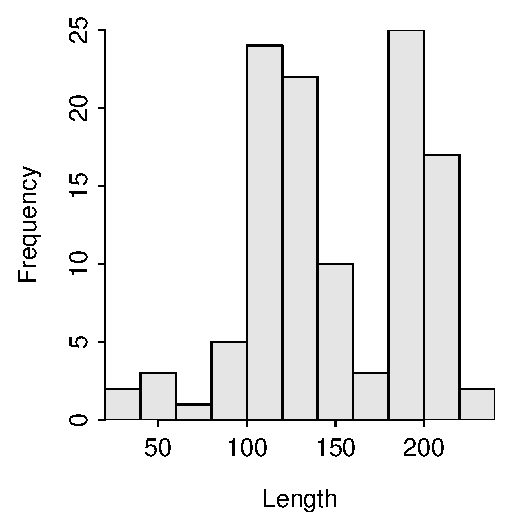
\includegraphics[width=.4\linewidth]{Figs/unnamed-chunk-1-1} 

}



\end{knitrout}
\begin{knitrout}
\definecolor{shadecolor}{rgb}{0.969, 0.969, 0.969}\color{fgcolor}\begin{kframe}
\begin{verbatim}

 f  m 
70 30 
\end{verbatim}
\end{kframe}
\end{knitrout}
\begin{knitrout}
\definecolor{shadecolor}{rgb}{0.969, 0.969, 0.969}\color{fgcolor}\begin{kframe}
\begin{verbatim}
The correlation is 0.975
\end{verbatim}
\end{kframe}

{\centering 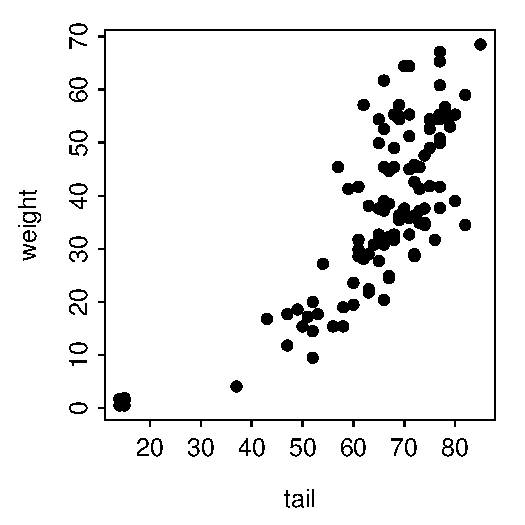
\includegraphics[width=.4\linewidth]{Figs/unnamed-chunk-3-1} 

}



\end{knitrout}
\begin{knitrout}
\definecolor{shadecolor}{rgb}{0.969, 0.969, 0.969}\color{fgcolor}\begin{kframe}
\begin{verbatim}
(Intercept)          tl 
  1.2604711   0.6157089 
The predicted value at a median of 125.85 is 78.747
The residual is 70 - 75.146 = -5.146
The r-squared value is 0.867
\end{verbatim}
\end{kframe}
\end{knitrout}

\clearpage
\begin{knitrout}
\definecolor{shadecolor}{rgb}{0.969, 0.969, 0.969}\color{fgcolor}\begin{kframe}
\begin{verbatim}
            
              f  m
  Allouez    15  6
  Interstate 13  7
  Whaleback  14  5
            
                f   m
  Allouez    14.7 6.3
  Interstate 14.0 6.0
  Whaleback  13.3 5.7
\end{verbatim}
\end{kframe}
\end{knitrout}
\begin{knitrout}
\definecolor{shadecolor}{rgb}{0.969, 0.969, 0.969}\color{fgcolor}\begin{kframe}
\begin{verbatim}
Pearson's Chi-squared test with table(rm$loc, rm$sex) 
X-squared = 0.3813, df = 2, p-value = 0.8264
\end{verbatim}
\end{kframe}
\end{knitrout}
\begin{knitrout}
\definecolor{shadecolor}{rgb}{0.969, 0.969, 0.969}\color{fgcolor}\begin{kframe}
\begin{verbatim}
Levene's Test for Homogeneity of Variance (center = median)
      Df F value Pr(>F)
group  1  0.0989 0.7543
      58               
\end{verbatim}
\end{kframe}
\end{knitrout}
\begin{knitrout}
\definecolor{shadecolor}{rgb}{0.969, 0.969, 0.969}\color{fgcolor}\begin{kframe}
\begin{verbatim}
 Two Sample t-test with bg by sex 
t = -0.4124, df = 58, p-value = 0.3408
alternative hypothesis: true difference in means is less than 0 
95 percent confidence interval:
     -Inf 5.246924 
sample estimates:
mean in group f mean in group m 
       78.47619        80.19444 
\end{verbatim}
\end{kframe}
\end{knitrout}

\end{document}
